\documentclass[11pt]{article}
\usepackage[scaled]{helvet}
\renewcommand\familydefault{\sfdefault} 
\usepackage[T1]{fontenc}%%% use with PDFLaTeX
\usepackage[utf8]{inputenc}
\usepackage[top=25mm,left=25mm,right=25mm,bottom=20mm,headsep=15pt,footskip=15pt,a4paper]{geometry} % see geometry.pdf on how to lay out the page. There's lots.
\usepackage[english]{babel}
\usepackage{color}
\usepackage{enumitem}
\usepackage[colorlinks,citecolor=blue]{hyperref}
\usepackage[parfill]{parskip} % no indentation
\newcommand\todo[1]{\textcolor{red}{#1}}
\usepackage[backend=biber,style=authoryear]{biblatex}
\emergencystretch=1em
\usepackage{graphicx}
\usepackage{amsmath}
\usepackage{amssymb}
\graphicspath{ {./figures/} }
\usepackage{wrapfig}
\addbibresource{references.bib}


\makeatletter         
\def\@maketitle{   % custom maketitle 
\begin{center}%
{\bfseries \@title}%
{\bfseries \@author}%
\end{center}%
\smallskip \hrule \bigskip }


\title{{\LARGE Coreference Resolution}\\[1.5mm]
{\large Working Title, First Draft: Content, not Wording}\\[1.5mm]} %%% Span Representation And Long-Range Coreference
\author{Patrick Kahardipraja, Olena Vyshnevska}%%% Fill in your name 
\date{} % delete this line to display the current date


%%% BEGIN DOCUMENT
\begin{document}

\maketitle


\section{Introduction}

% Role of Coreference Resolution in NLP . 
%Some nice long paragraphs about place of coreference in NLP  
Coreference Resolution (CR) is a vital part of Natural Language Understanding and Natural Language Processing (NLP). It's applications include information extraction, question answering, summarization, machine translation, dialog systems etc. The task consists of mention detection and mention clustering. Some systems only focus on one part, while others propose end-to-end solutions.

The notion of mention -- a span of text referring to some entity -- is central to the task of CR. Mentions can be one of the three kinds: pronouns, named entity, and noun phrases. When several mentions \textit{corefer} they refer to the same entity. 

Since the seventies automated solutions for coreference resolutions have been researched \parencite{woods1972, winograd1972, hobbs1978}. Some of the challenges central to the field include semantic and syntactic agreement between mentions; encoding non-local dependencies; paraphrasing of repetitions.


% While being a language short of elaborate agreements, English certainly enjoys the most scientific attention. It is a known challenge in NLP to do more research with agreement-rich languages \textit{citation needed}. 

% Challenges in the Field . 
% Paragraphs about problems with coref   
% Narrow down to loca/non-local coreference . 

% Our Proposed Solution
% Very broadly what we intended to to

Since the introduction of pre-trained BERT model  \parencite{devlin2019bert} there has been a lot of research showing how the model outperforms previous state-of-the-art task-specific NLP models. \todo{cite some papers here} % cite more papers here 
\textcite{joshi2019coref} has introduced BERT models into coreference resolution tasks. However, the researchers have also encoded other information on top of BERT embeddings. 

Our first research question is based on the recent research which shows that the BERT model itself encodes a significant amount of semantic and syntactic information. Therefore, we decided to test how well the span representations using BERT embeddings from the model by \textcite{joshi2019coref} finetuned on Ontonotes dataset \parencite{conll}  can encode coreference resolution information without any layers of additional information about a given sequence. 

As a baseline, we used original pre-trained BERT embeddings. To encode a mention span,  we used a convolutional layer and a  self-attention layer.

Our second research question, which naturally follows from the first one, whether the span representations encoded with a pre-trained BERT model simply modelling local coreference? Will it be able to encode non-local coreference dependencies? 

We found that the span represenations from within the coreference model by \textcite{joshi2019coref} reach \textit{insert some numbers}. The baseline model is at \textit{insert numbers}. This findings suggests that the pre-trained BERT model is a powerful tool for encoding information relevant to coreference resolution. 

For our second research question (non-local VS local dependencies) we found that ... \todo{what we found for local non-locat}

Our code is publicly available on GitHub.  \footnote{\url{https://github.com/alyonavyshnevska/bert_for_coreference_resolution}}.


\section{Related Work}

\subsection{Approaches to Coreference Resolution}
% Explain several types of approaches for coreference resolution with each difference, later link that we choose span-ranking models.

Architectures for coreference resolution models are typically categorized as 1) mention-pair classifiers \parencite{ng2002identifying, bengtson2008understanding}, 2) mention-ranking classifiers \parencite{durrett2013easy, wiseman2015learning, clark2016deep}, 3) entity-level models \parencite{haghighi-klein-2010-coreference, wiseman-etal-2016-learning}, or 4) latent-tree models \parencite{fernandes-etal-2012-latent, martschat-strube-2015-latent}.
Earlier solutions have been feature-based, while in the recent years neural classifiers have been particularly successful.

Nowadays a widely-adopted approach to coreference resolution are end-to-end models that perform mention detection, anaphoricity, and coreference jointly \parencite{jurafsky2019}. Beforehand, the rule-based systems were in use. Notable mentions are work by \textcite{hobbs1978}, \textcite{lappin1994}. \textcite{hobbs1978} invented a tree-search algorithm for identifying reference with robust results, which started a long series of syntax-based methods.  \textcite{lappin1994} combined syntactic and other features by assigning weights to those features and summing these up to score candidate mentions. \textcite{kennedy1996} optimised the approach to avoid full syntactic parsing. 

\textcite{yang2003coref} and \textcite{iida2003incorporating} helped establish mention-ranking approaches as influential solutions in the early 2000's. \textcite{ng2005b} pioneered the rise of end-to-end solutions. While rule-based systems have witnessed a short-lived revival in 2010s \parencite{zhou2004, haghighi2009}, their struggles with semantic understanding for the models led to their eventual demise.  The rise of neural architectures that dominated the NLP in the recent decade has inevitably established itself in coreference. 

\subsection{State of the Art Coreference Models}
%end-to-end and higher order
%bert, bert for coref

\begin{figure}[ht]
  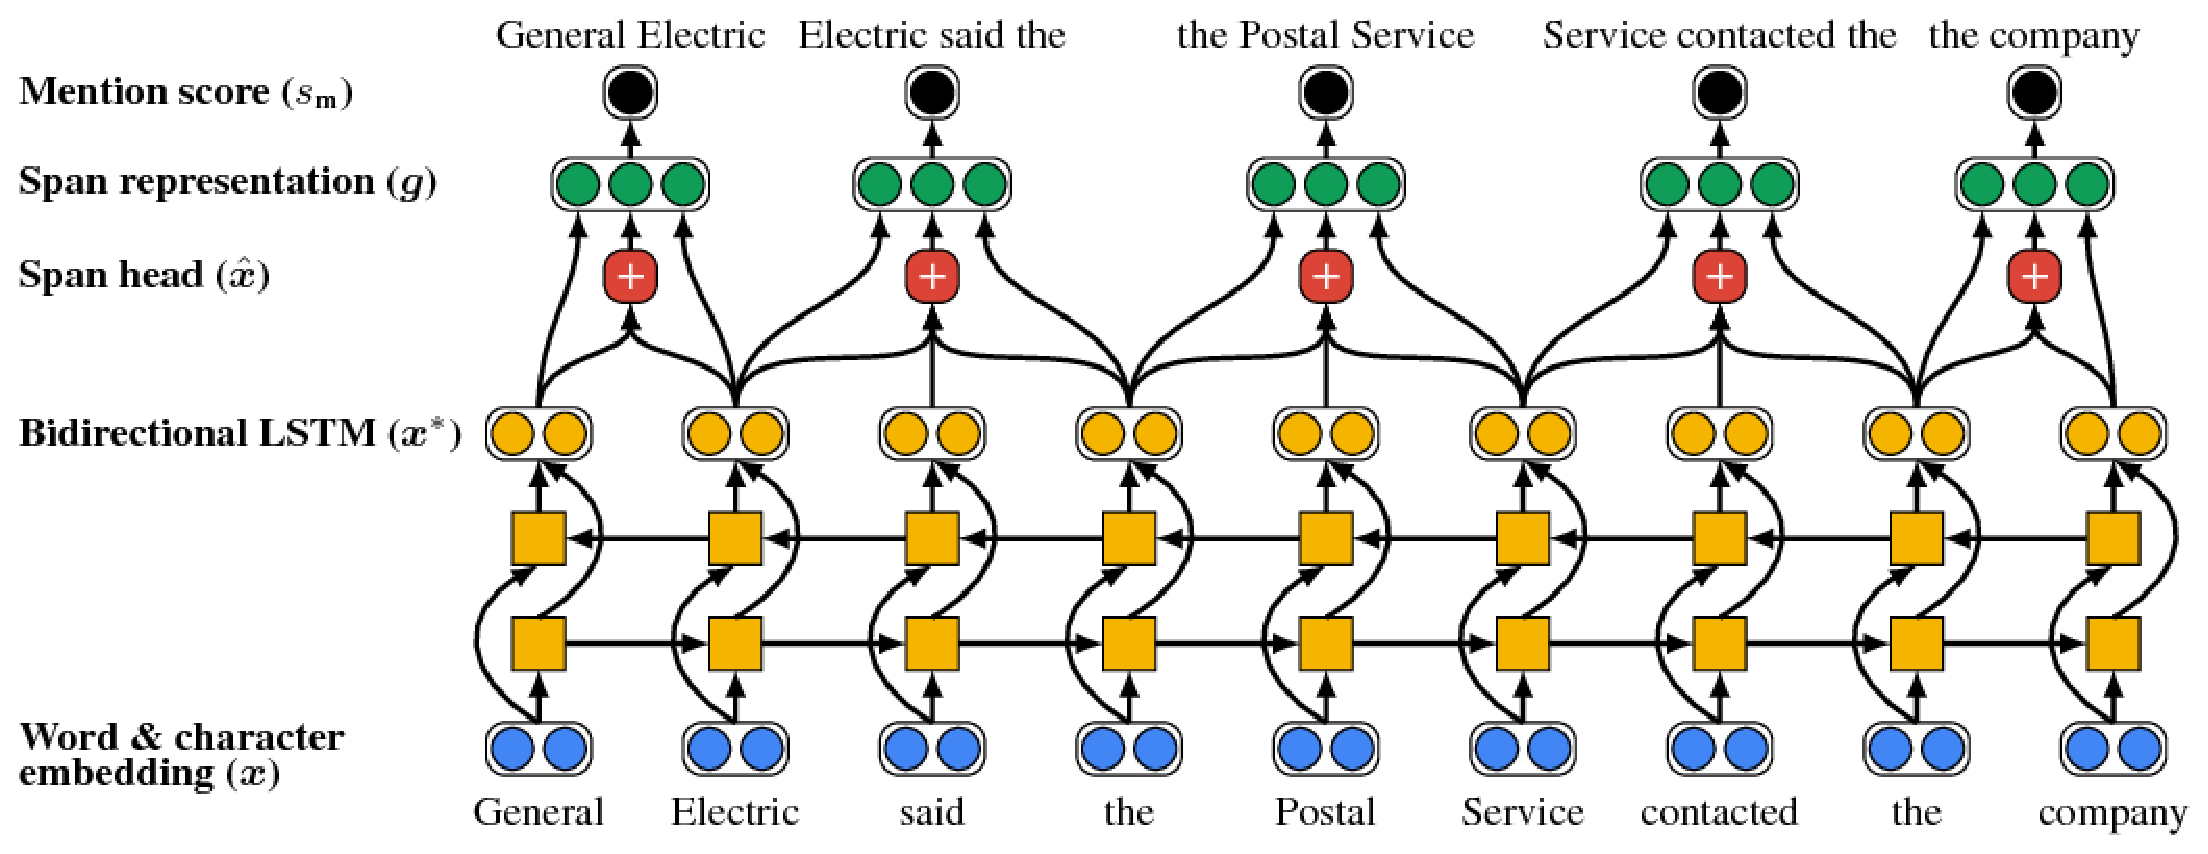
\includegraphics[width=\textwidth]{e2emodel.eps}
  \caption{Figure 1: First step of the end-to-end coreference resolution model, which computes embedding representations of spans for scoring potential entity mentions. Low-scoring spans are pruned, so that only a manageable number of spans is considered for coreference decisions. In general, the model considers all possible spans up to a maximum width, but we depict here only a small subset. \parencite{lee2017end}}
  \label{fig:e2emodel}
\end{figure}

\textcite{lee2017end} have proposed an span-ranking approach, which the authors describe as most similar to mention ranking, with reasoning over a larger space by detecting mentions and predicting coreference jointly in one end-to-end model. We will further refer to the model as \textit{e2e-coref}.


The authors showed that from the space of all possible spans their model implicitly  learns to produce meaningful mention candidates. A head-finding attention mechanism also learns a task-specific preference for head words, which has a strong correlation with head-word definitions in rule-based systems.

\begin{wrapfigure}{r}{0.5\textwidth} %this figure will be at the right
    \centering
      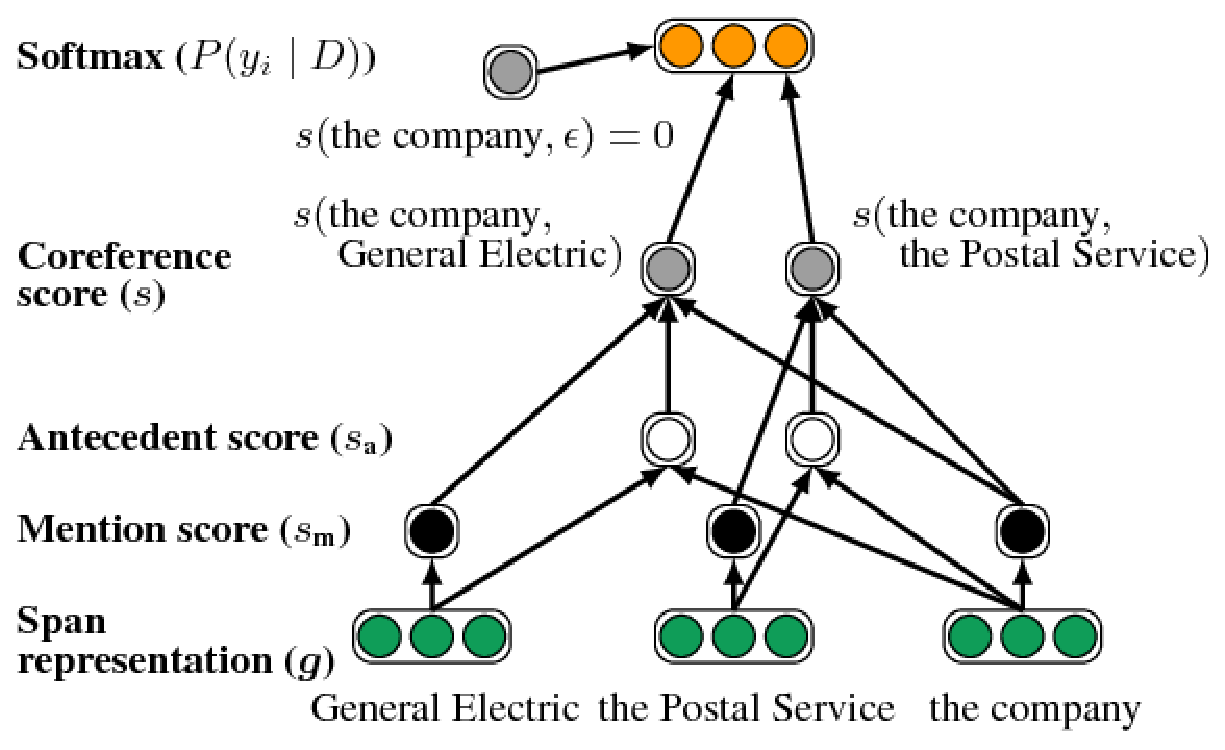
\includegraphics[width=0.5\textwidth]{e2e_extra_info.eps}
  \caption{Second step of end-to-end model by \textcite{lee2017end}. Antecedent scores are computed from pairs of span representations. The final coreference score of a pair of spans is computed by summing the mention scores of both spans and their pairwise antecedent score.  }
  \label{fig:e2e_extra_info}
\end{wrapfigure}

Building on to of the span-ranking neural architechture in \textcite{lee2017end}, \textcite{lee2018higher} proposed a model that captures higher order interactions
between spans in predicted clusters. We will further refer to this model as \textit{c2f-coref}. It also alleviates the additional computational cost of higher-order inference due to a coarse-to-fine approach, which allows the model to at first compute a rough sketch of likely antecedents, and only at a later stage apply a more exhaustive inference. Hence, the coarse-to-fine approach expands the set of coreference links that the model is capable of learning. 

To encode the span representations \textcite{lee2017end} use bidirectional LSTM \parencite{lstm} to encode the lexical information of the inside and
outside of each span. \textcite{lee2018higher} additionaly use the newly published ELMo embedding representations by \textcite{peters2018elmo} at the input to the LSTMs.

\textcite{joshi2019coref} took the architechture of \textcite{lee2018higher} and improved the performence of the model further by replacing the LSTM-based encoder with the BERT transformer \textcite{devlin2019bert}. We further refer to the model by \textcite{joshi2019coref} as \textit{bert-coref}.

\textcite{devlin2019bert} made a significant break-through with their pre-trained BERT model. It can be finetuned with one additional output layer
to create state-of-the-art models for a wide
range of NLP tasks, such as question answering and language inference, without substantial taskspecific architecture modifications. BERT's training examples consist of 128 and 512 word pieces. Such passage-level training has been an important improvement over the previous methods. It helps the model learn dependencies over text sequences longer than one sentence, such as the previous state of the art model ELMo \parencite{peters2018elmo}. Two model sized have been presented by \textcite{devlin2019bert}:
BERT-base(12 transformer blocks, hidden size 768, 12 self-attention heads, total Parameters=110M) and BERT-large (24 transformer blocks, hidden size 1024, 16 self-attention heads, total Parameters=340M).

%Figure \ref{fig:boat1} shows a boat.
\begin{figure}[h]
  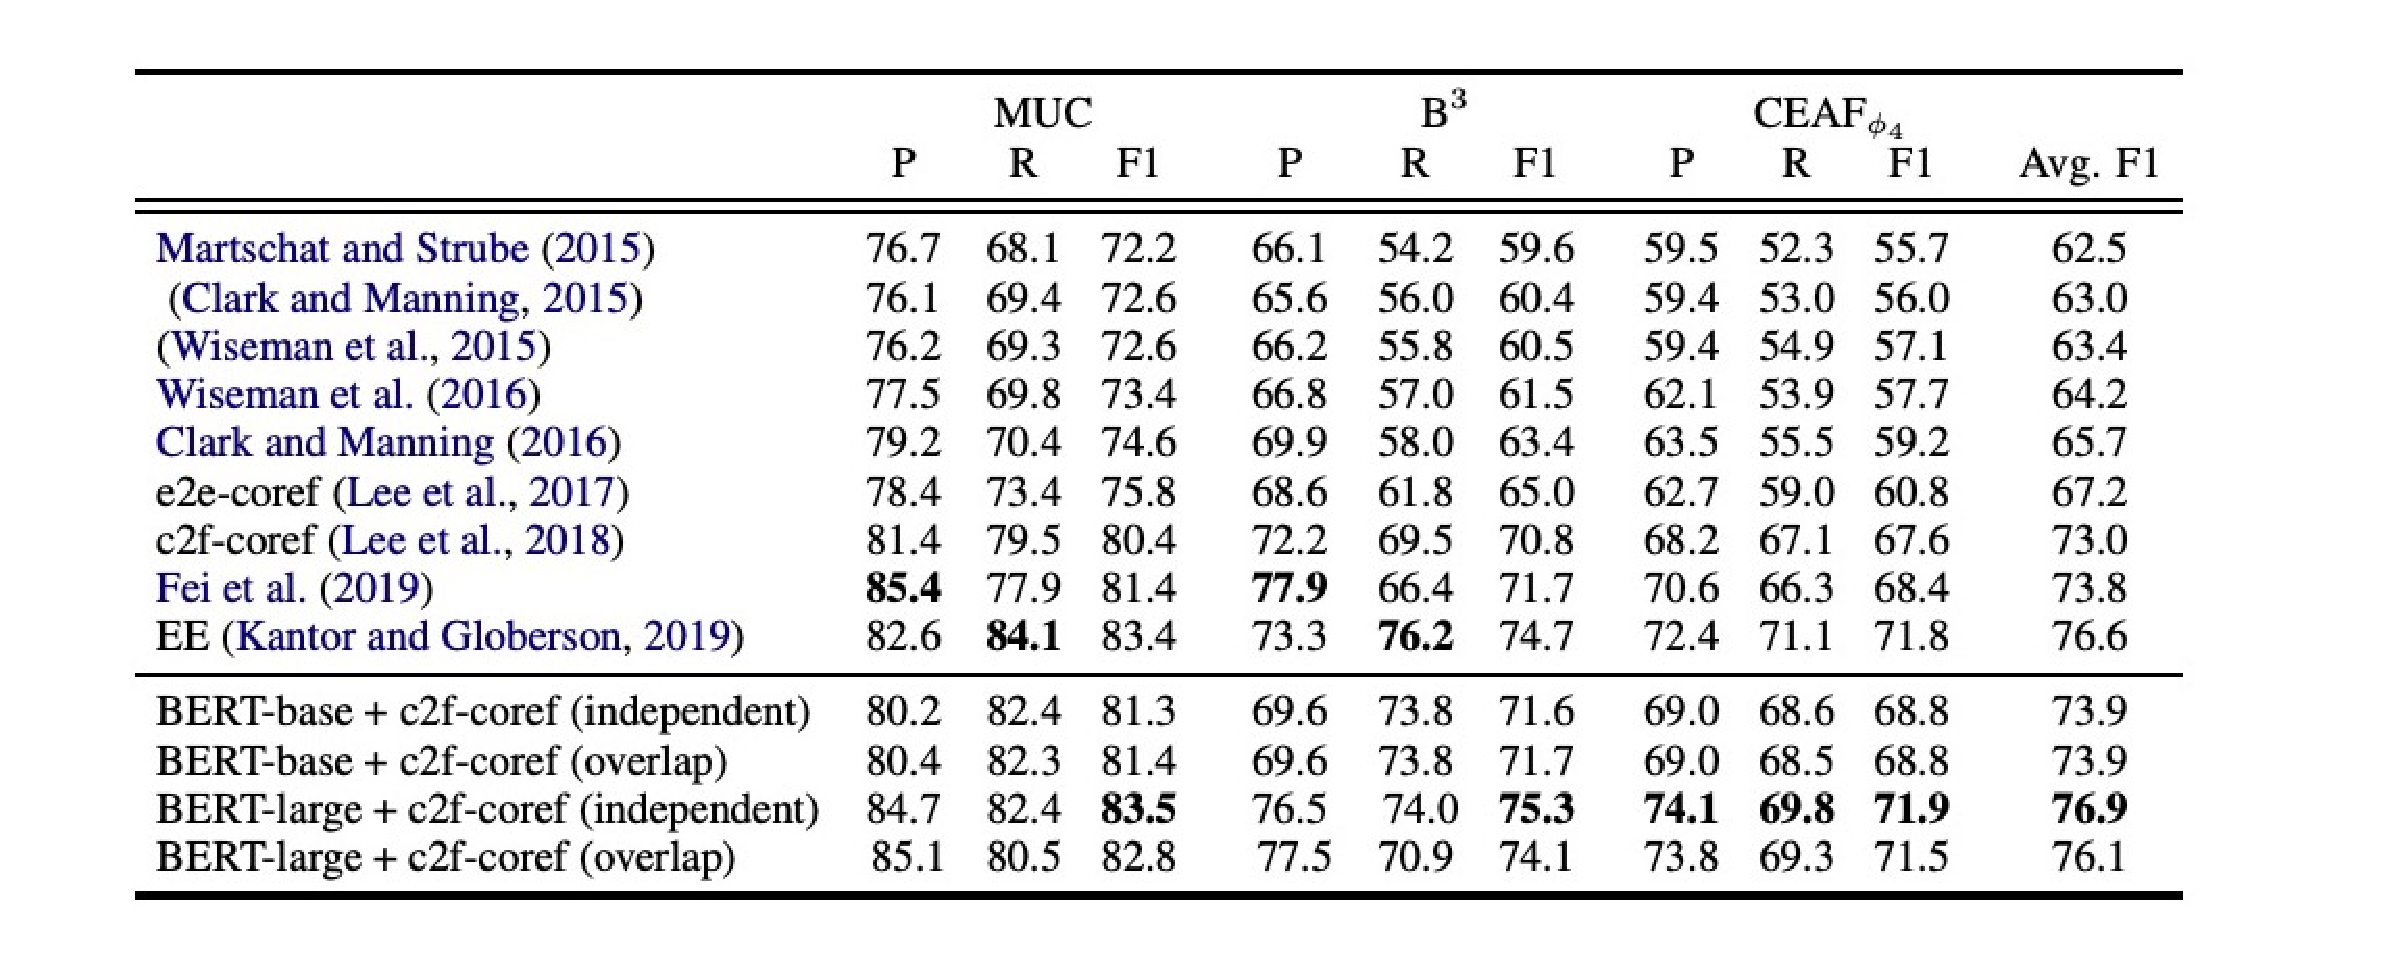
\includegraphics[width=\textwidth]{joshi_results.eps}
  \caption{OntoNotes: BERT improves the c2f-coref model on English by 0.9\% and 3.9\% respectively for base and large variants. \parencite{joshi2019coref}}
  \label{fig:joshiresults}
\end{figure}

\textcite{joshi2019coref} treat the first and last word-pieces in a mention (concatenated with the
attended version of all word pieces in the span) as span representations. The researchers test both models with BERT-base and BERT-large transformers. With this change to the c2f-coref model the authors gain an additional 3.9\% improvement on the OntoNotes compared to the already high results of \textcite{lee2018higher}. A quantitative analysis is shown in  figure \ref{fig:joshiresults}. 
A qualitative analysis done by the authors suggests that BERT-large (unlike BERT-base) is significantly better at distinguishing between related yet distinct entities or concepts.


\subsection{Coreference Arc Prediction Task}
% \textcite{liu2019linguistic}  Ling Knowledge and Transfer, Negative Samples, arc prediction task



Recently, there has been interesting work done to simplify state-of-the-art task-specific NLP models. 
 \textcite{liu2019linguistic} show evidence that frozen contextual represenations of word sequences fed into linear models can show similar levels of performance as state-of-the-art task-specific models on many NLP tasks.
The authors use probing models, also known as auxiliary or diagnostic classifiers \parencite{shi2016string, kadar2017representation} to analyse the linguistic information within contextual word representations. To test how the probing model performs in comparison to ELMo, the authors tested the models on a coreference arc prediction task, where the model predicts whether two mentions corefer. The Ontonotes dataset was used. To train the probing model the authors generate negative examples, where mentions that do not corefer are fed into the probing model alongside the mentions that do corefer. In our work we will also build our experiments similar to coreference arc prediction tasks suggested by the authors.

%\textcite{tenney2019context} Probing Model
\textcite{tenney2019context} introduced edge probing task design. For coreference resolution, the models had to determining whether two spans of tokens refer to the same entity. In order to investigate how good the contextual word representation models can model long-range dependencies, the authors used a fixed-width convolutional layer on top of the word representations to build spans of word pieces. The authors concluded that using the CNN layers on top of BERT-large pretarined model has performed particularly well on difficult semantic tasks, such as coreference resolution. Hence, in out work we will also follow the approach of the authors to construct our baseline. 
% and found that existing models trained on language modeling and translation produce strong representations for syntactic phenomena, but only offer comparably small improvements on semantic tasks over a non-contextual baseline. 

\section{Overview of End-to-End Span-ranking Model}
% Move Lee 2017, Lee 2018, Joshi 2019 here, with a more in-depth explanation, separate it from Related Work

\section{Probing Mention-span Representations}
% change section name to Probing Span Representations
% include overview of SOTA-architecture with BERT, preferably before the Probing Span Representations section
% Explain about Span Representations/Embeddings, especially regarding the features, define the span representations in SOTA

% Explain about the probing task, in this case Arc Prediction
% Explain about OntoNotes datasets, possibly can be moved to Experiments.
% Explain about probing model, possibly can be moved to Experiments. Explain also what is the input

\subsection{Span Representation}
\label{subsection:spanreps}

Span representation plays an important role in span-ranking model \parencite{lee2017end}, since it is used to compute distribution over candidate antecedent spans. In order to be able to predict coreference relations accurately, span representation should also capture the information of the span's internal structure and its surrounding context. In our experiments, we use the span representation which is first proposed in \parencite{lee2017end}, but with BERT \parencite{devlin2019bert} instead of a LSTM-based encoder to encode lexical information of the span and its surrounding, following \parencite{joshi2019coref}. The span representation is a vector embeddings which consists of context-dependent boundary representations with attentional representation of the head words over the span. The boundary representations are composed of first and last word-pieces of the span itself. The head words are automatically learned using additive attention [Bahdanau 2015] over each word-pieces in the span:
\begin{align*}
\alpha_{t} &= \pmb{w}_{\alpha} \cdot \text{FFNN}_{\alpha}(\pmb{x}_{t}^{*}) \\ 
a_{i,t} &=  \frac{exp(\alpha_{t})}{\sum\limits_{k=start(i)}^{end(i)} exp(\alpha_{k})} \\ 
\hat{\pmb{x}}_{i} &= \sum\limits_{t=start(i)}^{end(i)} a_{i,t} \cdot \pmb{x}_{t}
\end{align*}

where $\hat{\pmb{x}}_{i}$ is a weighted vector representation of word-pieces for span $i$. This representation is augmented by a $\mathbb{R}^{d}$ feature vector which encodes the size of span $i$ with $d = 20$. The final representation $\pmb{g}_{i}$ for span $i$ is formulated as the following:
\begin{align*}
\pmb{g}_{i} = [\pmb{x}_{start(i)}^{*}, \pmb{x}_{end(i)}^{*}, \hat{\pmb{x}}_{i}, \phi_{i}]
\end{align*}  

where $\pmb{x}_{start(i)}^{*}$ and $\pmb{x}_{end(i)}^{*}$ are first and last word-pieces of the span, and $\phi_{i}$ is the span width embeddings.

\subsection{Coreference Arc Prediction}
\label{subsection:corefarc}

%Span representations will be then used as inputs for coreference arc prediction task \cite{liu2019linguistic}, where a probing model (in this case a simple FFNN) is used to predict coreference relations. The probing model is designed with limited capacity to focus on what information that can be extracted from the span representations. The probing model itself has a sigmoid output layer, which is trained to minimize binary cross entropy. Each negative samples (\textit{w\_entity}, \textit{wb}) will be generated for every positive samples (\textit{wa}, \textit{wb}) where \textit{wb} occurs after \textit{wa} and \textit{w\_entity} is a token that occurs before \textit{wb} and belong to a difference coreference cluster, to ensure a balanced data. By comparing the performance of the probing model using span representations, we can hypothesize to what extent that the proposed span representation in \textcite{joshi2019coref}  can capture coreference information. We will also experiment with mention span separation distance to see how the probing model performs and whether if there is a degradation of accuracy and F1 score of the probing model with distant spans.


% Tenney focus on span, Liu focus on CWR
We focus on coreference arc prediction task, which is a part of probing tasks suite for contextual word embeddings \parencite{liu2019linguistic, tenney2019context}. In this task, a probing model is trained to determine whether if two mentions refer to the same entity. As datasets for coreference resolution usually only contains annotations for corefering mentions, we produce negative samples following the approach by \parencite{liu2019linguistic}. For every pair of mentions $(w_{i}, w_{j})$, where they belong to the same coreference cluster and $w_{i}$ is an antecedent of $w_{j}$, we generate a negative example $(w_{random}, w_{j})$ where $w_{random}$ belongs to a different coreference cluster. This method ensures that the ratio between positive and negative examples is balanced. We also follow the approach of \parencite{tenney2019context} by using spans of word-pieces for mentions, as \parencite{liu2019linguistic}'s approach is limited on single-token mentions and therefore unable to fully exploit the information in the mention-span.


\subsection{Probing Model}
% add box to indicate frozen part!
\begin{figure}[ht]
  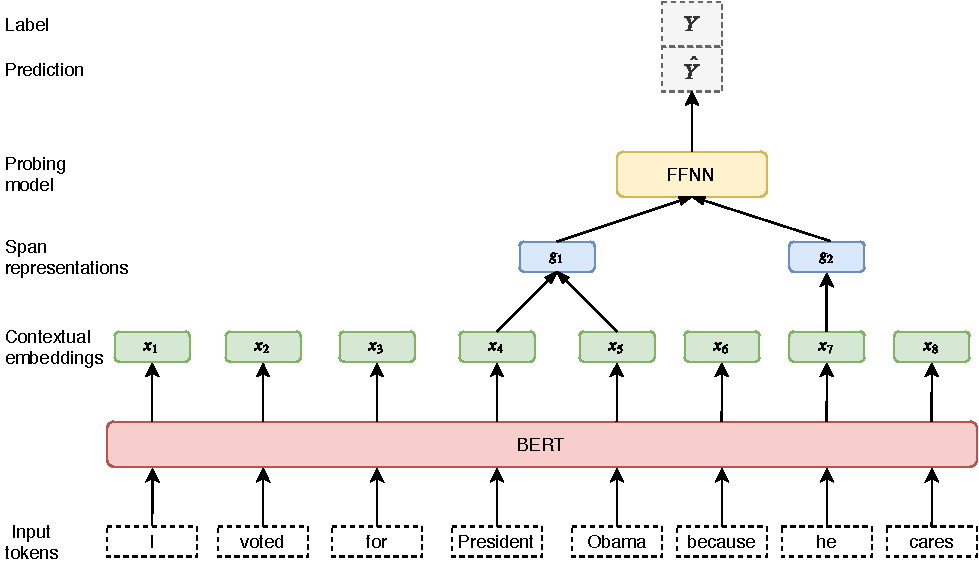
\includegraphics[width=\textwidth]{probing_model}
  \caption{Probing architecture for span representation. The feed-forward neural network is trained to extract information from the span representations $\pmb{g}_{1}$ and $\pmb{g}_{2}$, while all the parameters inside the dashed line are frozen. The example depicts a mention-pair, where $\pmb{g}_{1}$ corresponds to span representation of "President Obama", while $\pmb{g}_{2}$ corresponds to "he". We predict $\hat{Y}$ as positive for this example.}
  \label{fig:probing_model}
\end{figure}

Our probing model is a simple feed-forward neural network, which is designed with a limited capacity to focus on what information that can be extracted from the span representations.
As the input to our probing model, we take the span representation for pair of mention-spans $\pmb{g}_{1} = [\pmb{x}_{start(1)}^{*}, \pmb{x}_{end(1)}^{*}, \hat{\pmb{x}}_{1}, \phi_{1}]$ and $\pmb{g}_{2} = [\pmb{x}_{start(2)}^{*}, \pmb{x}_{end(2)}^{*}, \hat{\pmb{x}}_{2}, \phi_{2}]$, where both $\pmb{g}_{1}$ and $\pmb{g}_{2}$ are concatenated together and passed to the FFNN. The FFNN consists of a single hidden layer followed by a sigmoid output layer. The model is trained to minimize the binary cross-entropy with respect to the gold label $Y \in \{0,1\}$. The probing architecture is shown in Figure \ref{fig:probing_model}.
\pagebreak
%Draw figure ffnn with positive and and negative examples ala tenney

% Explain using BERT-finetuned on OntoNotes and non-finetuned, base and large cased
We explore mention-span representations obtained from BERT. BERT \parencite{devlin2019bert} is a language representations model which uses deep Transformer architecture [Vaswani 2017], trained jointly with masked language model and next sentence prediction objective on BooksCorpus [Zhu et al 2015] and English Wikipedia, with an approximate total of 3,300M tokens. It also enables significant improvement in many downstream tasks with relatively minimal task-specific fine-tuning. To study the quality of mention-span representations, we extract mention-span embeddings from BERT-base (12-layer Transformer, 768-hidden) and BERT-large (24-layer transformer, 1024-hidden). We also want to compare the effect of fine-tuning BERT-based models on the quality of span representations, therefore we use two variant of BERT models: a) fine-tuned on coreference resolution task and b) without any fine-tuning.



\section{Experiments}
% Explain that we do 2 experiments, first to see how the architectures improves span representation compared to non-finetuned BERT embeddings. Second one is to see long-range coreference phenomena.
% Explain pre-trained contextualized word embeddings that we used in the project, in this case BERT fine-tuned on OntoNotes and BERT which is not-fine tuned, use BERT-base and BERT-large cased, with 128 and 384 max segment length, because it is the best results. Independent variant
% Implementation and hyperparams
% Introduce baseline models here, also explain a bit regarding the attention..
% Explain how we see the long-range coference phenomena, with span separation distance.

% Move this to experiment
%We attempt to investigate 1) to what extent the span representations proposed using span embeddings with BERT \parencite{devlin2019bert} in \textcite{joshi2019coref} can encode coreference information, 2) and whether it is able to encode non-local coreference phenomena or is it just simply modeling local coreference.

%In order to analyse the first research question, we experiment with BERT-based span representations in \textit{bert-coref} model. The model is finetuned on OntoNotes. A single span represenattion for a mention consists of BERT embeddings for its first and last word-pieces concatenated with the attention version of all word pieces in the span. These span embeddings are a part of a larger \textit{bert-coref} model. \textcite{joshi2019coref} calculate several scores on top of span representations: mention score, antecedent score, and coreference score, which is then passed through a softmax layer. \ref{fig:e2e_extra_info} illustrates these additional layers. 

% move this part to analysis?
%For our research we refer to the work of \textcite{liu2019linguistic}. The research argue that frozen contextual represenations of word sequences fed into linear models can show similar levels of performance as state of the art task-specific models on many NLP tasks. We are interested in analysing how BERT span representations fed into a linear model will perform on a coreference task. For our experiments we will use a similar strategy as the coreference arc prediction task proposed by t\textcite{liu2019linguistic}.

%We extract the BERT span representations from a pipeline provided in a GitHub repository by \textcite{joshi2019coref} \footnote{\url{https://github.com/mandarjoshi90/coref}}. 

We attempt to investigate to what extent the proposed span representation using BERT embeddings and fine-tuned on corefence resolution task can encode coreference relations. We also want to answer whether if the span representation is able to encode long-range coreference phenomena effectively, or is it just simply modeling local coreference relation? Our experiments, which we describe below, are intended to analyze coreference information contained in the span representation used in the span-ranking model. 

\subsection{Dataset}
% REPHRASE THIS LATER, DON'T FOLLOW JOSHI
For our experiments, we use the coreference resolution annotation
from the CoNLL-2012 shared task based on the OntoNotes dataset \parencite{conll}. The dataset comprises of roughly one million words from various genre such as newswire, magazine articles, broadcast news, broadcast conversations, web data and conversational speech data, and the New Testament in English, which was splitted into 2802 training documents, 343 validation documents, and 348 test documents. On average, the training documents contain 454 words. The largest document contains a maximum of 4009 words. Beside entities, coreference is also annotated for mentions that refer to the same event (e.g. "The European economy \textbf{grew} rapidly over the past years, \textbf{this growth} helped raising...).The main evaluation of the dataset is the average F1 score of three metrics – $MUC$ [Vilain 1995], $B^3$ [Bagga and Baldwin 1998] and $CEAF_ \phi4$ [Luo 2015]. Since OntoNotes only provide annotations for positive examples, we generate our own negative examples according to the aforementioned method (\S \ref{subsection:corefarc}). We also cast the original annotation provided in the dataset into JSON format in order to work with BERT-coref. 
% we work with jsonlines format by joshi, also mention the number of train, test, dev after casting?

\subsection{Implementation and Hyperparameters} 
%We extract the span representations from the coreference model by \textcite{joshi2019coref}. The model has been fine tuned on OntoNotes English data for 20 epochs using a dropout of 0.3, and learning rates of $1 * 10 ^{-5}$ and $2 * 10 ^{-4} $ with linear decay for the BERT parameters and the task parameters respectively. A batch size of 1 document has been used. 

We extend the original Tensorflow implementation of BERT-coref \footnote{\url{https://github.com/mandarjoshi90/coref}} in order to build our probing model with Keras frontend [cite Keras]. Our probing model are trained for 50 epochs, using early stopping with patience of 3 and batch size of 512. For optimization, we use Adam [Kingma and Ba] with a learning rate of 0.001. The weights of the probing model is initialized with Kaiming initialization [Kaiming] and the size of the hidden layer is $d=1024$ with ReLU activation function.

As mentioned previously, we use both original pre-trained BERT model without fine-tuning the encoder weights and BERT model that has been fine-tuned on coreference resolution task (i.e. on OntoNotes annotations). For fine-tuned BERT model, we take the models that yield the best performance on \parencite{joshi2019coref}, which were trained using 128 word-pieces for BERT-base and 384 word-pieces for BERT-large. The fine-tuned model was trained using splitted OntoNotes documents where each segment non-overlaps and fed as a separate instance. This is done as BERT can only accept sequences of at most 512 word-pieces and typically OntoNotes documents require multiple segments to be read entirely. In all of our experiments, we use the cased English BERT models.
% original BERT

\subsection{Baseline}
%As our baseline, w euse pre-trained BERT embeddings (not finetuned on OntoNotes) for all tokens within the mention span, which is then passed through a convolutional layer (with kernel width of 3 and 5) to incorporate the local context and followed by self-attention pooling operator to produce a fixed-length span representations. This is to model head words, inspired by approach from \textcite{tenney2019context}.

%max span width 30

%pooling is only within bounds of span, means that the only information our model can access about the rest of the sentence is provided by contextual embeddings of words within the span

% Describe span representation for baseline too! and padding part

As our baseline model, we use span representations introduced in the edge probing framework \parencite{tenney2019context}. We take concatenated contextual embeddings for pair of mention-span $e^{(1)} = [x_{1}^{(1)}, x_{2}^{(1)}, x_{3}^{(1)}, ..., x_{n}^{(1)}]$ and $e^{(2)} = [x_{1}^{(2)}, x_{2}^{(2)}, x_{3}^{(2)}, ..., x_{n}^{(2)}]$ as inputs. We then use a shared projection layer, which is followed by the self-attention pooling operator in (\S \ref{subsection:spanreps}) to produce a fixed-length span representations and model head words for each mention-span. These mention-span representations are then passed to the probing model to predict whether they corefer or not. It is important to note that the self-attention pooling is computed only using tokens within the boundary of the span. As a result, the model can only access information about the context surrounding the mention span through the contextual embeddings. We take the word-piece embeddings from activations of BERT final layer, while freezing the encoder. The baseline probing architecture is depicted in Figure ...

%explain why the baseline is as it is

\subsection{Long-range Coreference}
%In order to answer our second research question is whether the span representations encoded with a pre-trained BERT model simply modelling local coreference and will it be able to encode non-local coreference dependencies. In order to answer it, we bucket the test data into separate groups based on the the length of the coreference distance between the a mention and antecedent. We do separate qualitative and quantitative analysis on the buckets in order to analyse the differences in performance of our models based on how large the distance is. 


% Add this after discussing baseline and long-range coreference
% The resulting representations have a dimension of d=768 or 1024.


\section{Results}
% Relate that it is possible to eliminate second step of the model? Seeing that probing model can be enough to predict coreference links?

% We generate representation from the encoder and train model to make predictions from those features alone. If a simple model can be trained to predict coreference from the span representation alone, we can reasonably conclude that the span representation encode this information
\begin{itemize}
\item some nice plots here
\item some tables here
\end{itemize}

\section{Discussion}

\begin{itemize}
\item long long analysis of what we've seen
\item generalisations, parallels
\item what do this results tell us about coref and nlp in general
\item discussion of why they are the way the are
\end{itemize}

We found that the model by \textcite{joshi2019coref} has performed very well. 
However, since the research is heavily based on the English language, it may be a phenomena particular to this language. The nominal declension in Ukrainian, for example, has seven cases; adjectives, pronouns have gender specific forms. Therefore, a similar analysis should be done for other languages before one can generalize the findings universally. % maybe it's more relevant in the conclusion

A benefit of using neural models for coreference resolution is their ability to use
word embeddings to capture similarity between words, a property that many traditional feature-based models lack.

\subsection{Future Work}
\begin{itemize}
\item everything we don't have the time for
\item mention other corpora that could be used for finetuning (Winogrande, GAP...)
\item apply roberta, etc.

\end{itemize}

\section{Conclusion}

\begin{itemize}
\item so what have we learned about coref in general and local dependencies in particular
\end{itemize}
\newpage % bibliography should start on new pages for nicer formatting, can delete this if space is not enough. keep it for now.
\printbibliography

\end{document}

% https://www.overleaf.com/learn/latex/Articles/Getting_started_with_BibLaTeX

%\textcite{joshi2019coref} bert for coref

%\textcite{lee2018higher} Higher-Order

%\textcite{lee2017end} End-to-End

%\textcite{devlin2019bert} Bert



